\documentclass{article}
\usepackage[T1]{fontenc}
\usepackage{lmodern}
\usepackage{graphicx}
\usepackage{amsmath,amssymb}
\usepackage[a4paper,margin=2cm]{geometry}
\usepackage[absolute,overlay]{textpos}
\setlength{\TPHorizModule}{1mm}
\setlength{\TPVertModule}{1mm}
\usepackage[indonesian]{babel}
\usepackage{hyperref}
\setlength{\emergencystretch}{2em}
% unit: Halaman 41

\begin{document}

% === Halaman 41 (llm) ===

\section*{Elliptic Curve Diffie-Hellman (ECDH)}

\begin{itemize}
    \item \textbf{Public:} Kurva eliptik dan titik $B(x,y)$ pada kurva
    \item \textbf{Secret:} Integer milik Alice, $a$, dan integer milik Bob, $b$
\end{itemize}

\vspace{40mm}

\begin{itemize}
    \item Alice menghitung $K = a \cdot (b.B)$
    \item Bob menghitung $K = b \cdot (a.B)$
    \item Hasil perhitungan akan sama karena $ab = ba$
\end{itemize}

\vspace{5mm}

\textcolor{red}{(*) Sumber bahan: \textcolor{red}{Debdeep Mukhopadhyay}, \textcolor{red}{Elliptic Curve Cryptography}, \textcolor{red}{Dept of Computer Sc and Engg IIT Madras}}

% deskripsi: Diagram pertukaran kunci ECDH antara Alice dan Bob yang menunjukkan pengiriman nilai publik a.B dan b.B
% bbox normalisasi: [0.1800, 0.3400, 0.7900, 0.6300]
\begin{textblock*}{128.10mm}(37.80mm,100.98mm)
\noindent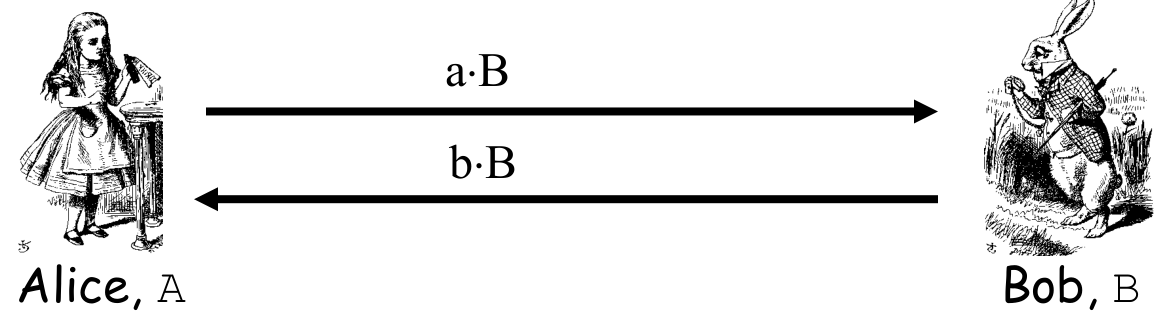
\includegraphics[width=128.10mm,height=86.13mm]{../../images/llm/page_041_img_01.png}%
\end{textblock*}

\end{document}
